Finite size targets interacting with high-intensity coherent radiation are a well-studied phenomenon of linearly excited
surface plasmon oscillations. Absorption and scattering of incident light in this case can be described with good accuracy using the Mie theory, which predicts the existence of a resonance corresponding to multipole oscillations of a part of the free electrons of the target relative to positively charged ions. In the resonance regime, effective excitation of surface plasmons can lead to a significant enhancement of the internal and external fields at the natural frequency of the cluster. This can lead to amplification of the field scattered at large angles relative to the initial direction of the incident wave.

Within micrometer wavelengths, photonic crystals and gratings can be used to guide or diffract electromagnetic waves~\cite{lin_zhang}, while similar X-ray manipulations can use crystals with atoms regularly spaced a few nanometers apart, as scattering centers~\cite{batterman_cole}. At the same time, a large gap between these wavelength ranges, called XUV (extreme-ultraviolet) or hard ultraviolet, turns out to be difficult to manipulate.

It is well-known fact that high-order laser harmonics can be generated using a short intense laser pulse when interacting with dense solid surfaces~\cite{teubner_gibbon_hoh}. In the intensity range under consideration (order of $10^{18}$ $\textrm{W/cm}^2$), the conversion coefficient is at best about $10^{-4}$, which gives the intensity of high-order harmonics no higher than $10^{14 }$ $\textrm{W/cm}^2$, which is not enough to ionize the target and generate plasma with a purely imaginary refractive index. To solve this problem, it is proposed to use a prepulse.

\begin{tikzfigure}
    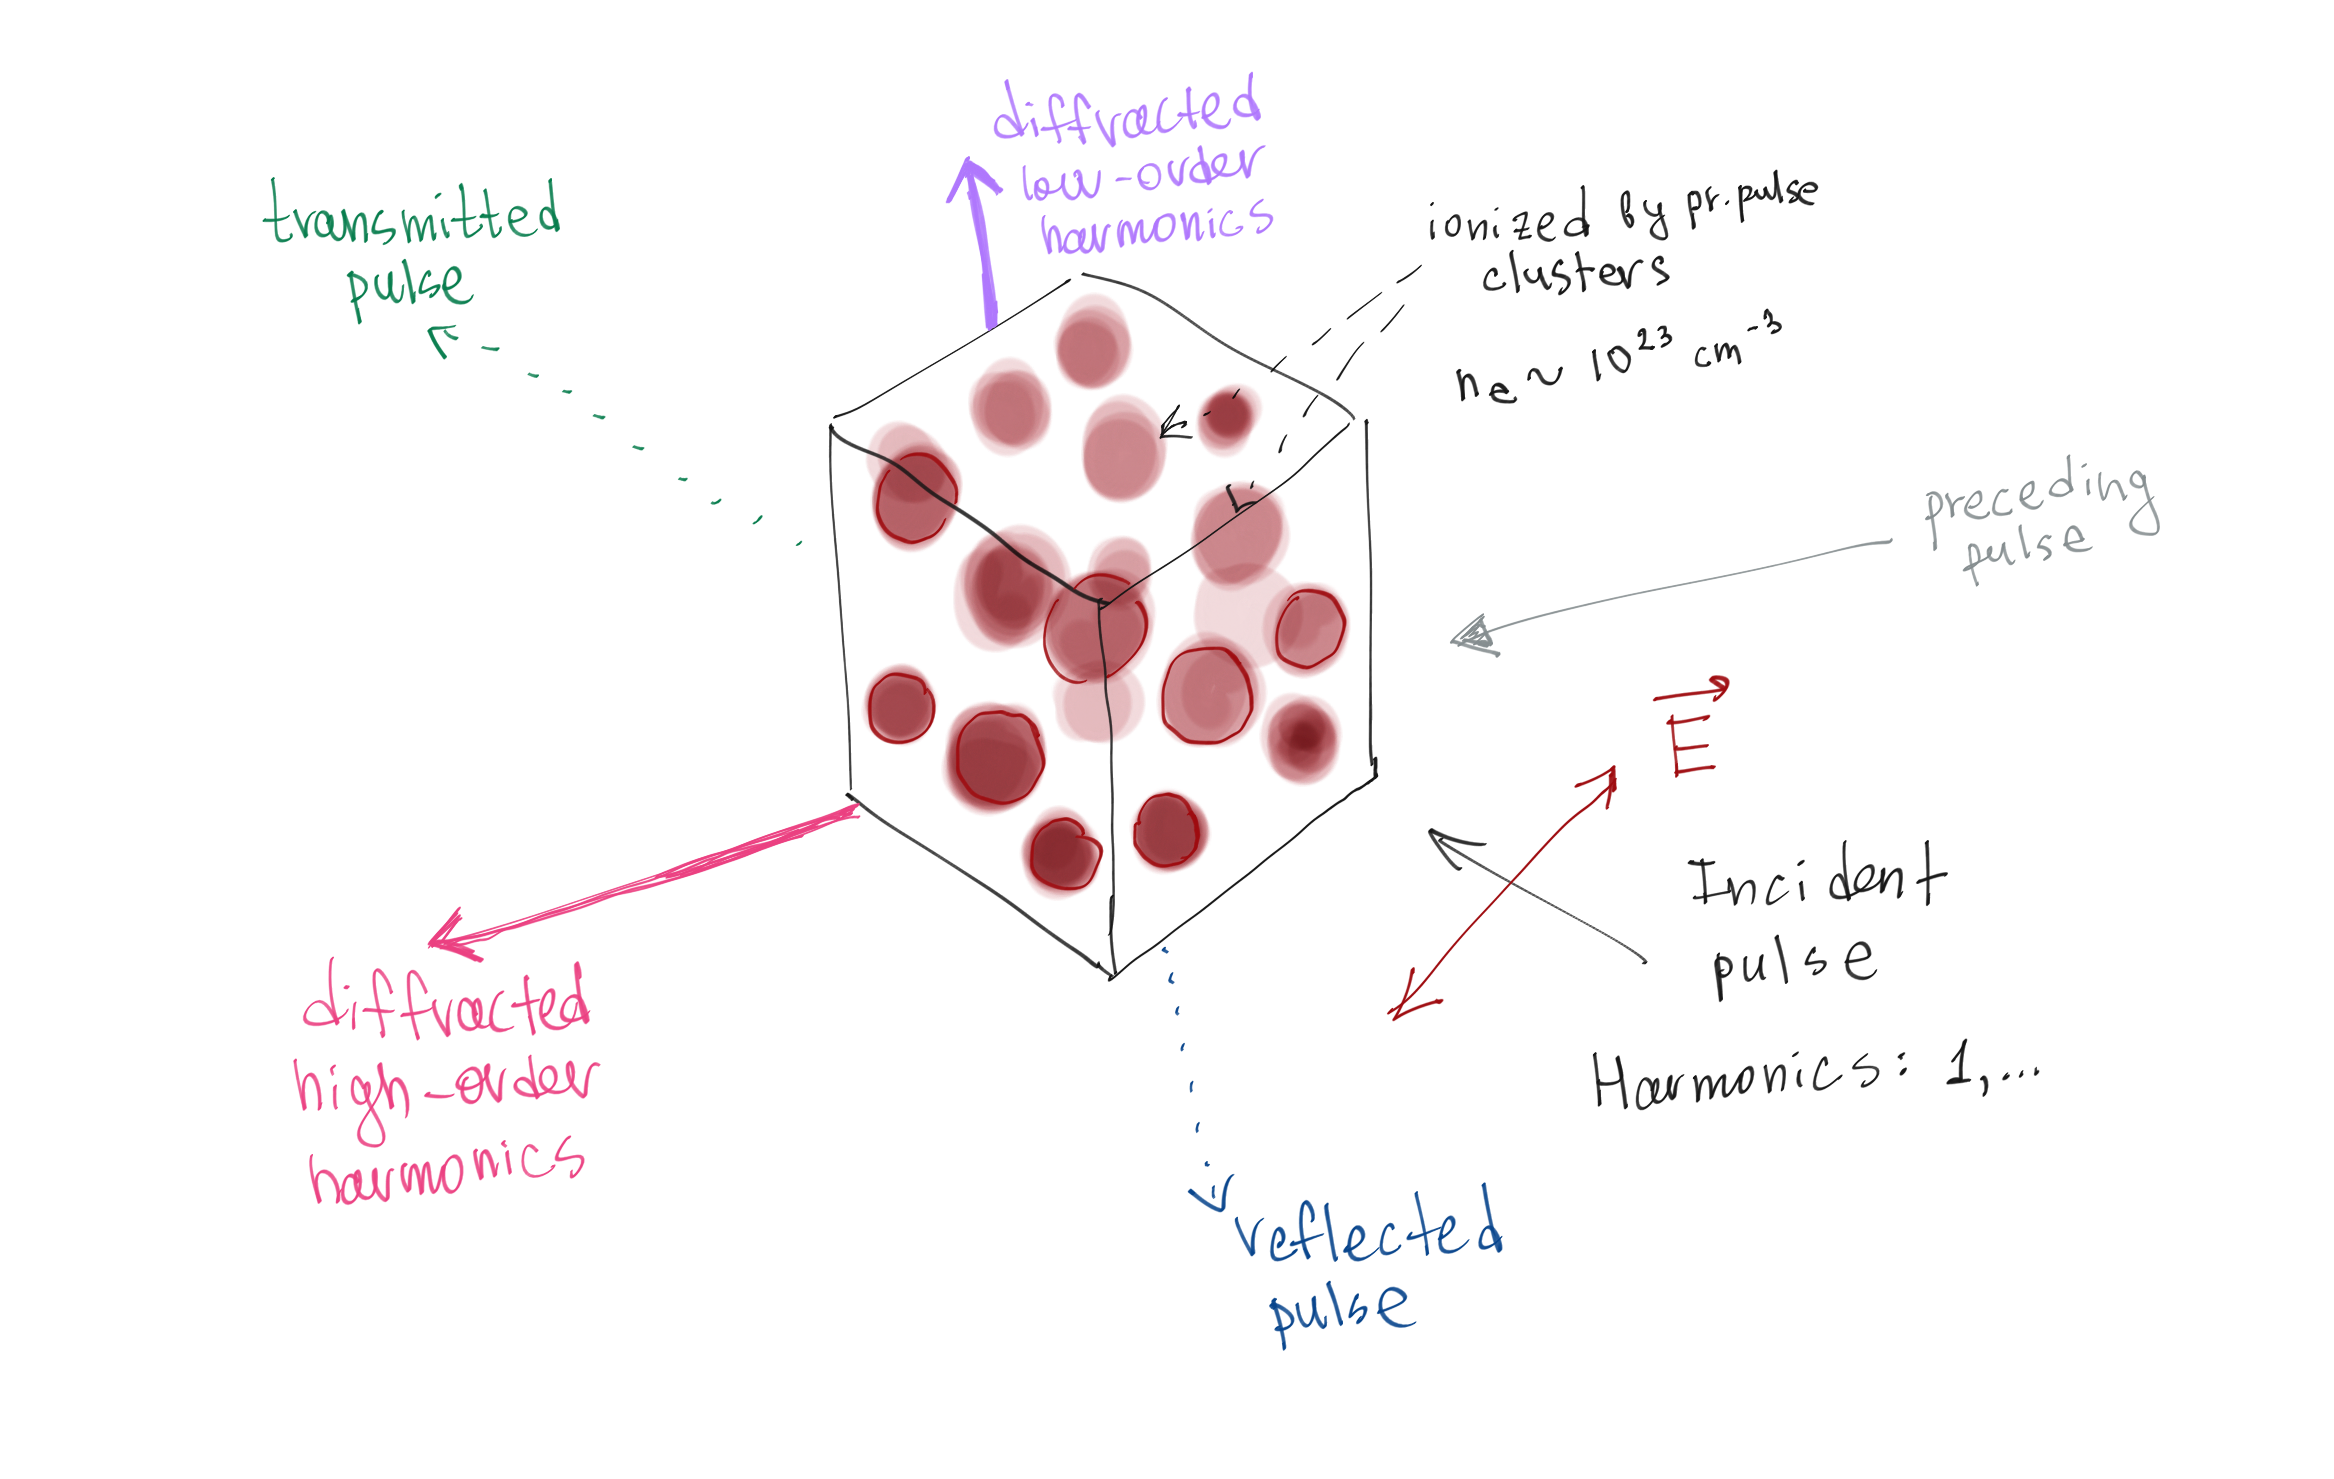
\includegraphics[width=0.9\linewidth]{../components/img/plasma_area2}\label{intsch:image}\caption{An interaction scheme. The plane of polarization is parallel to one of the faces of the cubic region. The sizes of spherical clusters are on the order of a few nanometers, and the distance between them is at least hundreds of nanometers. The distribution of clusters inside the cubic region is generally arbitrary, the clusters do not intersect the faces of the region.}
\end{tikzfigure}

A generalized interaction scheme is shown in Fig.~\ref{intsch:image}. The harmonics that the main pulse contains have different intensities at different angles, which leads to an angular dependence of the output radiation shape.


%Рассеяние одиночным сферическим кластером с хорошей точностью описывается в рамках теории Ми, поэтому такое линейное приближение предлагается использовать и в случае множества кластеров с целью качественной оценки и дальнейшего уточнения при помощи PIC моделирования (метод частиц-в-ячейках).

% \img[components/img/plasma_area2]{Схема взаимодействия. Плоскость поляризации параллельна одной из граней кубической области. Размеры сферических кластеров порядка единиц нанометров, расстояния между ними не менее сотни нанометров. Распределение кластеров внутри кубической области в общем случае произвольно, кластеры не пересекают грани области.}{plasma_area1:image}{0.8\textwidth}